\section{Analysis} \label{sec:analysis} 

As it is shown in section~\ref{sec:evaluation}, Adjacency Filtering reduces the
number of edit-distance calls a lot. However, as the Adjacency Filtering will
always test if \textit{N - e} segments match to corresponding locations, the
effectiveness of Adjacency Filtering is related to the user-defined error
tolerance number \textit{e}. As \textit{e} increases, the effectiveness of
Adjacency Filtering decreases, since the required number of matching segments
is reduced.  To maintain the Adjacency Filtering effectiveness, one solution
will be using shorter key for hash table thus cut the fragments into shorter
segments and increasing the segments count. For example, if the fragment is 108
base-pairs in length and each segment is 12 base-pair in length so we cut the
fragment into 9 segments, for a user set error tolerance number \textit{e=5},
instead of requiring \textit{N-e = 9-5 = 4} segments find corresponding
adjacent locations, we now reduce the key length to 9 which will divide the
fragment into 12 segments, and we will require \textit{N-e = 12-5 = 7} segments
finding corresponding adjacent locations. We have simulated 9 case for 1
chromosome and it turns out when \textit{e=5}, setting key length to 9 does
increase the effectiveness of Adjacency Filtering where it is filtering out
more not-matching locations. However, we do see a longer execution time. The
reason is that although the Adjacency Filtering effectiveness is enhanced, the
cost of Adjacency Filtering is also increased. Since now the keys are shorter
and the entries are fewer while the total number of coordinates stays the same
as before. As a result, the coordinate list for each hash table entry is
increased, which means Adjacency Filtering will need to traverse more
coordinates. To make it even worse, now there are more segments for each
fragments and thus more searching for corresponding adjacent coordinates. Last
but not the least, this increases the chance of encountering \textit{popular}
keys with the same reason we described in section~\ref{sec:algorithm}, as now
we have longer coordinate list. In all, shorter keys increases the execution
time a lot. In Figure~\ref{fig:c0912_af}, we show when changing key length from 12 to 9. How
many coordinate are subjects to Adjacency Filtering compared to before. In
Figure~\ref{fig:c0912_ed}, we show the increased effectiveness of Adjacency Filtering since
less coordinates will be subject to edit-distance calculation and Figure~\ref{fig:c0912_speed}
shows the increased execution time. \\ 

For cheap key selection, we face the same problem. Since we are picking the
cheapest \textit{N-e+1} keys. As \textit{e} increases, the keys we pick will
become less \textit{cheap}. When \textit{e = N-1}, the program will just behave
as if without cheap key selection, since it is picking all the keys anyhow. We
can increase the chance of picking relatively cheap keys by the same trick as
above: smaller key length and more segments. However, by the same reason above,
increasing the key number does not necessarily provides speed up. Although we
increase the chance picking relatively cheap keys, since the coordinate list is
longer now, the \textit{cheap} keys’ coordinate list are actually longer than
before. The results is shown in Figure~\ref{fig:c0912_af} as well.

In reality, normally error tolerance \textit{e} is set to 5\% of the fragment
sequence length. For a 108 read, \textit{e} will normally be 5, by which
FashHASH still provides generally considerable speed up. However, as \textit{e}
increases, the performance improvement will diminish, because of the reason
stated above. \\

%%%%%%%%%%%%%%%%%%%%%%%%%%%%%%%%%%%%%%%%%%%%%%%%%%%%%%%%%%%%%%%%%%%%%%%%%%%%%%%%
\begin{figure}[h] \centering
\vspace{0.1in}
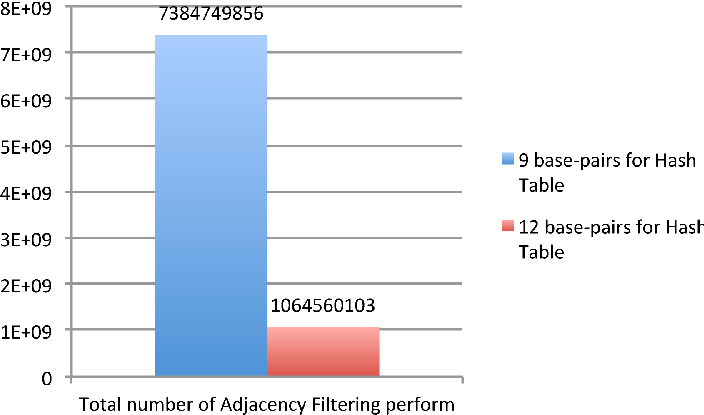
\includegraphics[height=1.8in]{./figure/C0912_AF_B.pdf} \vspace{0in}
\caption{The number of Adjacency Filtering performs \\
		(9 base-pairs Hash table vs. 12 base-pairs Hash table)}
\label{fig:c0912_af} \end{figure}
%%%%%%%%%%%%%%%%%%%%%%%%%%%%%%%%%%%%%%%%%%%%%%%%%%%%%%%%%%%%%%%%%%%%%%%%%%%%%%%%

%%%%%%%%%%%%%%%%%%%%%%%%%%%%%%%%%%%%%%%%%%%%%%%%%%%%%%%%%%%%%%%%%%%%%%%%%%%%%%%%
\begin{figure}[h] \centering
\vspace{0.1in}
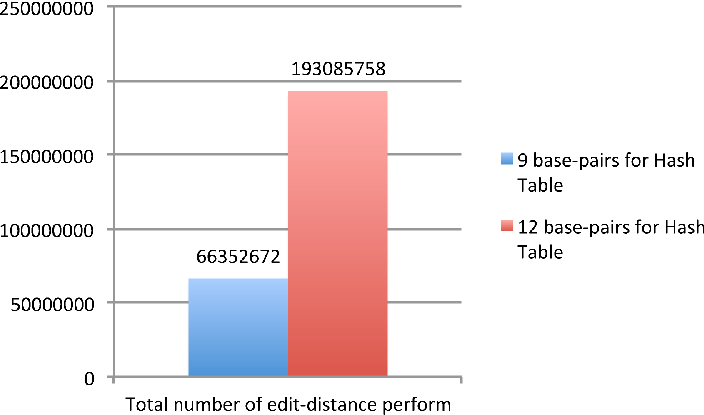
\includegraphics[height=1.8in]{./figure/C0912_ED_B.pdf} \vspace{0in}
\caption{The number of edit-distance calculation performs \\ 
		(9 base-pairs Hash table vs. 12 base-pairs Hash table)}
\label{fig:c0912_ed} \end{figure}
%%%%%%%%%%%%%%%%%%%%%%%%%%%%%%%%%%%%%%%%%%%%%%%%%%%%%%%%%%%%%%%%%%%%%%%%%%%%%%%%

%%%%%%%%%%%%%%%%%%%%%%%%%%%%%%%%%%%%%%%%%%%%%%%%%%%%%%%%%%%%%%%%%%%%%%%%%%%%%%%%
\begin{figure}[h] \centering
\vspace{0.1in}
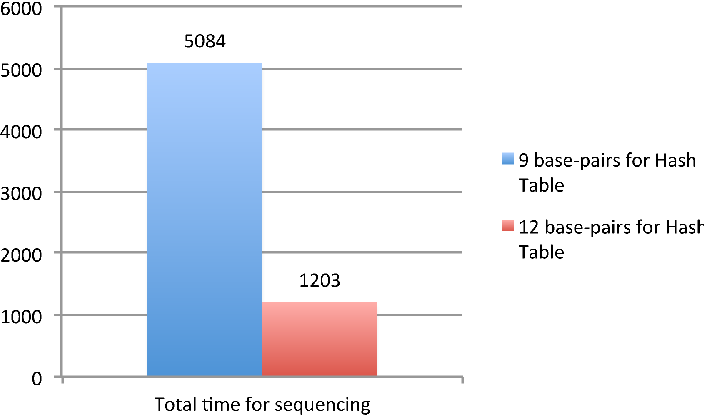
\includegraphics[height=1.8in]{./figure/C0912_Speed_B.pdf} \vspace{0in}
\caption{The sequencing speed \\ 
		(9 base-pairs Hash table vs. 12 base-pairs Hash table)}
\label{fig:c0912_speed} \end{figure}
%%%%%%%%%%%%%%%%%%%%%%%%%%%%%%%%%%%%%%%%%%%%%%%%%%%%%%%%%%%%%%%%%%%%%%%%%%%%%%%%

We also analyzed why GPU performed not as good. As stated in GPU implementation
section, the warp is not fully utilized. We write a simple GPU mimic function
that simulates the GPU warp and we show the result in Figure~\ref{fig:warp}. From the chart,
we can see that for most of the time, edit-distance calculation under utilize
the warp: for the majority of the warp execution, only 4 threads are active.
For Adjacency Filtering, the situation is slightly better, since about 1/9 of
the time, the warp is filled, but still this is not enough. Especially when for
the majority of the time there are only several threads are active.\\

%%%%%%%%%%%%%%%%%%%%%%%%%%%%%%%%%%%%%%%%%%%%%%%%%%%%%%%%%%%%%%%%%%%%%%%%%%%%%%%%
\begin{figure}[h] \centering
\vspace{0.1in}
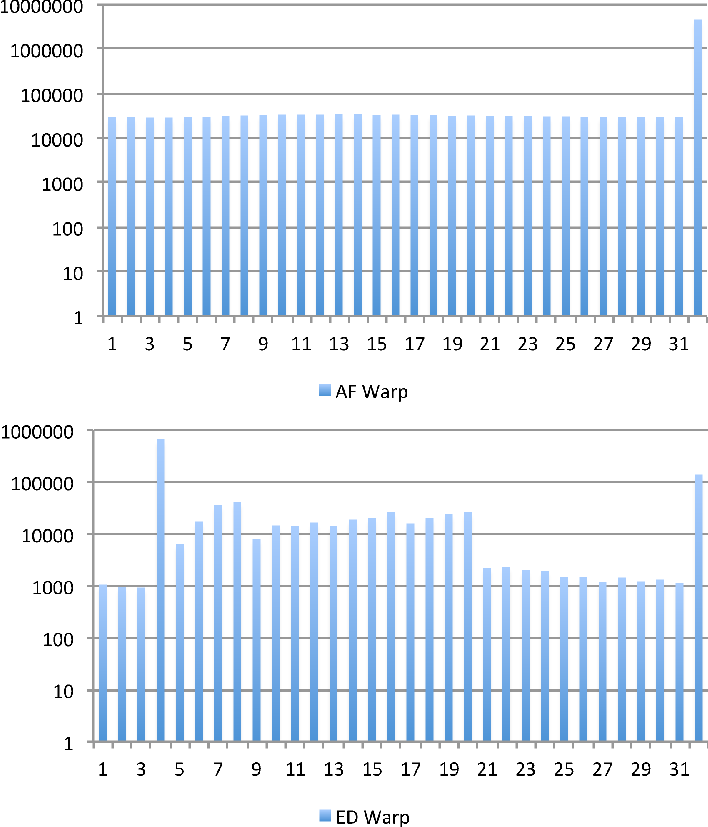
\includegraphics[width=3in]{./figure/Warp2_B.pdf} \vspace{0in}
\caption{GPU Analysis}
\label{fig:warp} \end{figure}
%%%%%%%%%%%%%%%%%%%%%%%%%%%%%%%%%%%%%%%%%%%%%%%%%%%%%%%%%%%%%%%%%%%%%%%%%%%%%%%%
